\documentclass[10pt,twosides]{book}
 
\usepackage{sty_files/BV}

\newif\ifdessins
\dessinsfalse
\newif\ifcouleur
\couleurfalse
\newif\ifpythontex
\pythontextrue

\usepackage{amsmath,amsfonts}
%\usepackage{mathabx}
\usepackage{tikz}
\usetikzlibrary{calc,shapes}

\renewcommand{\thesection}{\arabic{section}}
\renewcommand{\thesubsection}{\arabic{section}.\alph{subsection}}
\setcounter{secnumdepth}{3}
\renewcommand{\thesubsubsection}{\roman{subsubsection}}
\renewcommand\FrenchLabelItem{$\bullet$}

%% Rendre les guillemets ('�' et '�') actifs.
%%
%% Attention, cela implique de ne pas mettre d'espace apr�s '�'
%% ni avant '�' dans le code source.
%%
%% Exemple de composition correcte: �comme ceci�.

\catcode`\�=\active
\catcode`\�=\active
\def�{\og\ignorespaces}
\def�{{\fg}}

\newcommand{\ofg}[1]{\og{}#1\fg{}}
%\newcommand{\Z}[0]{\mathbb{Z}}
%\newcommand{\N}[0]{\mathbb{Z}}
%\newcommand{\R}[0]{\mathbb{Z}}
%\newcommand{\Q}[0]{\mathbb{Z}}
    % Import macros diverses

\tikzset{
    hexgrid/.style= {shape=regular polygon,regular polygon sides=6,minimum size=1cm, draw,inner sep=0,anchor=south,fill=white,rotate=30}
}
\tikzset{
    hexcell/.style= {shape=regular polygon,regular polygon sides=6,minimum size=1cm, draw,inner sep=0,anchor=south,fill=gray!50,rotate=30}
}

\newcommand{\hexgrid}[2]{
    \foreach \x in {0,...,#1} {
    \foreach \y in {0,...,#2} {
        \pgfmathparse{mod(\y,2)};
        \node[hexgrid]
            (h\x;\y) at (0.45*\pgfmathresult+1.75*\x*0.5,-1.5*\y*0.5) {};
    }
    }
}

\newcommand{\hexcell}[2]{
    \node[hexcell] at (h#1;#2.south) {};
}
\newcommand{\pivot}[2]{
    \fill[black] (h#1;#2.center) circle (2pt);
    \draw[black] (h#1;#2.center) circle (5pt);
}

\newcommand{\unit}[1]{
    \foreach \x/\y in {#1} {
        \hexcell{\x}{\y}
    }
}

\newcommand{\CW}[2]{
    \draw [->,very thick] (h#1;#2.center) ++(330:.2cm) arc (330:0:.2cm);
}
\newcommand{\CCW}[2]{
    \draw [->,very thick] (h#1;#2.center) ++(30:.2cm) arc (30:360:.2cm);
}
\newcommand{\mSE}[2]{
    \draw [->,very thick] (h#1;#2.center) ++(-60:.21cm) -- ++(-60:.5cm);
}
 % Import macros sp�cifiques grille hexagonale

\pagestyle{fancy}
\fancyhf{}

\fancyhead[RO]{\small  \leftmark \ \ {\bf \thepage}}
\fancyhead[LO]{\small  BV 252\ -- \ Automne 2015}
\fancyhead[RE]{\small  BV 252\ -- \ Automne 2015}
\fancyhead[LE]{\small  {\bf \thepage} \ \ \leftmark}
\fancypagestyle{plain}{%
\fancyhf{}
\renewcommand{\headrulewidth}{0pt}
\renewcommand{\footrulewidth}{0pt}
}%

  \renewcommand{\chaptermark}[1]{ \markboth{#1}{}}
    \uchyph=0


\begin{document}
\chapter{Participation � l'ICFP 2015}

\section{Introduction}

Marc de Falco a propos� durant l'�t� aux membres de l'UPS de participer au 
tournoi de programmation de l'ICFP\footnote{International Conference on 
Functional Programming} (voir \url{icfpcontest.org}) qui s'est tenu sur 
trois jours du vendredi 7 ao�t 2015 (14h) au lundi 10 ao�t 2015 (14h). � son 
appel, une �quipe (TaupeGoons) s'est form�e pour relever le d�fi. Elle �tait constitu�e 
de quatre membres:

\begin{itemize}
	\item	Marc de Falco, le GO du groupe qui a tout orchestr� et a abattu la 
	majorit� du travail;
	
	\item	Jean-Julien Fleck, qui s'est occup� de l'optimisation des 
	param�tres par algorithme g�n�tique ;
	
	\item	Laurent Jospin, qui malheureusement a d� d�clarer forfait suite � 
	des soucis informatiques ;
	
	\item	Lo�c Pottier, qui a d�velopper son propre moteur de r�solution et 
	a fini par former sa propre �quipe (GaupeToons), d'abord pour le tester, 
	puis pour essayer de l'am�liorer puisque les r�sultats �taient plut�t 
	bons.
	
\end{itemize}

Le pr�sent article vise � d�crire le probl�me pos� pour le tournoi ainsi que 
la mani�re dont l'�quipe TaupeGoons s'est ing�ni� � le r�soudre. Tout le code 
informatique utilis� peut �tre retrouv� � l'adresse

\begin{center}
\url{https://github.com/MarcdeFalco/icfp15}
\end{center}


\section{Probl�me pos�}

\subsection{Description rapide}
Le probl�me � r�soudre consiste � �crire un programme jouant tout seul � TETRIS$^\circledR$
sur une grille hexagonale.

L'ensemble des pi�ces � utiliser est propre � chaque plateau et la pi�ce � poser est d�termin�e
par un g�n�rateur pseudo-al�atoire fix�.

Chaque pi�ce pos�e de mani�re d�finitive (dans la suite on dira qu'elle a �t� \emph{v�rouill�e})
permet de marquer des points.

Chaque mouvement possible d'une pi�ce peut �tre repr�sent� par plusieurs caract�res et la solution
doit �tre pr�sent�e sous la forme d'une cha�ne de caract�res.

L'ambig�it� sur la repr�sentation d'un mouvement permet l'inclusion de mots intelligibles dans 
une solution tout en pr�servant son sens et son impact sur le plateau.

Dix-huit phrases sp�ciales peuvent �tre incluses dans les solutions pour gagner des points.

Il s'agit donc de jouer au mieux tout en faisant appara�tre le plus de phrases sp�ciales dans 
la solution.

\subsection{Plateau et syst�me de coordonn�e}
Le plateau est une grille hexagonale bidimensionnel de cellules.

Une cellule a deux �tats : \emph{libre} ou \emph{occup�e}.

Les rang�es de la grille sont dispos�es en quinconce et on en d�duit le syst�me de coordonn�es
suivant pr�sent� dans la figure~\ref{fig:hexcoord1}
\begin{figure}
    \caption{\label{fig:hexcoord1}Syst�me de coordonn�es pour la grille hexagonale}
\ifdessins
\centering
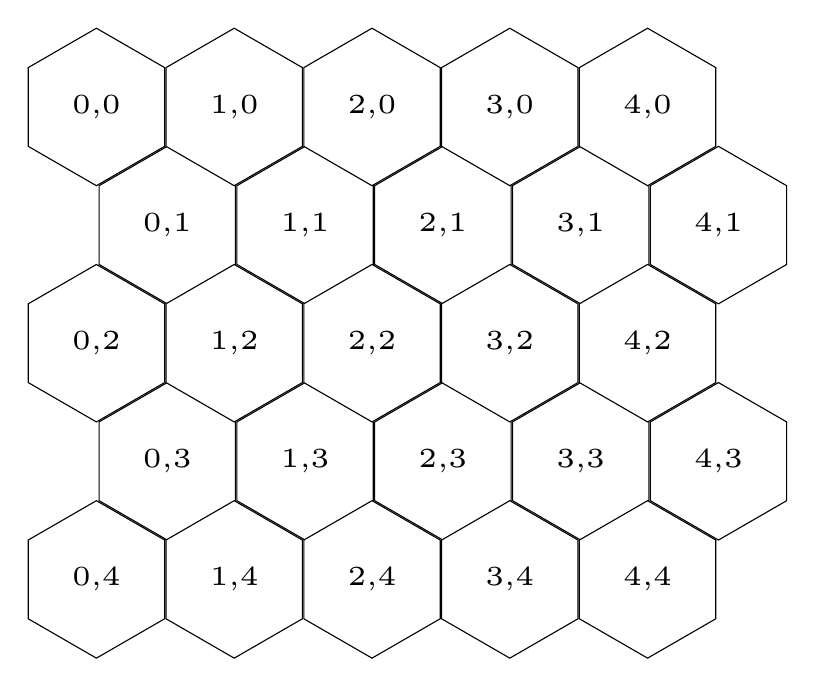
\begin{tikzpicture}[scale=2, every node/.style={transform shape}]
    \hexgrid{4}{4}
    \foreach \x in {0,...,4} {
    \foreach \y in {0,...,4} {
        \node at (h\x;\y.center) {\tiny \x,\y};
    }
    }
\end{tikzpicture}
\fi
\end{figure}

Notons tout de suite que ce syst�me de coordonn�es a le probl�me suivant : les d�placements
dans la grille ne sont pas proportionnel � des d�placements g�om�trique. En effet, si on souhaite passer effectuer une translation d'un cran en bas � droite (ce qui sera d�fini comme le mouvement
$\searrow$ au paragraphe~\ref{par:moves}) on ne peut pas se contenter d'ajouter $(1,1)$ 
aux coordonn�es car si le point $(4,7)$ devient effectivement $(5,8)$ apr�s cette translation,
le point $(4,6)$ devient $(4,7)$. Tout d�pend de la parit� de la rang�e sur laquelle un point
se situe.

\subsection{Pi�ces}
Une pi�ce est d�termin�e par un ensemble de cases qu'elle occupe en position neutre
et la donn�e d'un point sur la grille appel� son pivot, qui n'est pas n�cessairement 
une des cases occup�es et dont les coordonn�es peuvent sortir du plateau.

Voici des exemples de pi�ces o� les cases vides sont \ifcouleur color�es \else gris�es \fi
et le pivot est indiqu� par un cercle au centre de la cellule sur laquelle il se situe :
\ifdessins
\begin{center}
    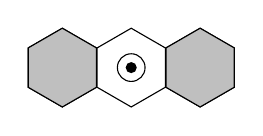
\begin{tikzpicture}
        \hexgrid{2}{0}
        \unit{0/0,2/0}
        \pivot{1}{0}
    \end{tikzpicture}
    \quad
    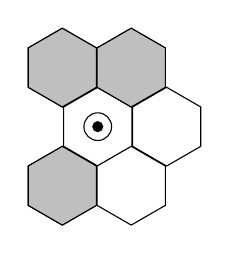
\begin{tikzpicture}
        \hexgrid{1}{2}
        \unit{1/0,0/0,0/2}
        \pivot{0}{1}
    \end{tikzpicture}
    \quad
    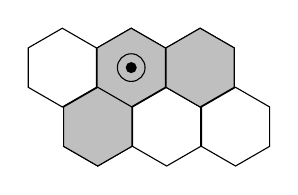
\begin{tikzpicture}
        \hexgrid{2}{1}
        \unit{2/0,1/0,0/1}
        \pivot{1}{0}
    \end{tikzpicture}
\end{center} 
\fi


\subsection{Donn�es initiales}
Chaque instance du probl�me � r�soudre est d�crit par un sextuplet 
$(w,h,\mathcal{O},N,\overline{g},\overline{p})$ o�
\begin{description}
    \item[$w\times h$] les dimensions du plateau
    \item[$\mathcal{O}$] l'ensemble des cases d�j� occup�es
    \item[$N$] le nombre de pi�ces � placer lors de chaque partie
    \item[$\overline{g} = (g_1,\dot,g_m)$] les germes des parties � jouer
    \item[$\overline{p} = (p_1,\dot,p_n)$] les diff�rents types de pi�ces disponibles.
\end{description}

\subsection{G�n�rateur pseudo-al�atoire}
Afin de d�terminer la pi�ce courante un g�n�rateur pseudo-al�atoire est utilis�
avec un germe donn� dans la description de l'instance.

On commence par d�finir la suite congruente lin�aire $(u_n)_{n\in \N}$
o� $u_0$ est le germe et 
\[
\forall n\in \N, u_{n+1} = (1103515245 u_n + 12345) \mod 2^{32}
\]

Le g�n�rateur pseudo-al�atoire $v_n$ correspond aux bits 16 � 30, en commen�ant � num�roter 0 le 
bit de poids faible, de la suite $u_n$. Soit avec une formule math�matique :
\[
\forall n \in \N, v_n = \left\lfloor \frac{u_n}{2^{16}} \right\rfloor \mod 2^{15}
\]

\subsection{Mouvements et verrouillage}
\label{par:moves}

Pour d�placer une pi�ce on dispose de six mouvements :
\begin{description}
    \item[$\sW$] mouvement d'un cran � gauche (Ouest)
    \item[$\sE$] mouvement d'un cran � droite (Est)
    \item[$\sSW$] mouvement d'un cran � gauche et d'un cran en bas (Sud-Ouest)
    \item[$\sSE$] mouvement d'un cran � droite et d'un cran en bas (Sud-Est)
    \item[$\sCCW$] rotation d'un angle $\frac{\pi}{3}$ autour du pivot 
        (Rotation anti-horaire)
    \item[$\sCW$] rotation d'un angle $-\frac{\pi}{3}$ autour du pivot 
        (Rotation horaire)
\end{description}

Un mouvement est valide si toutes les cellules occup�es apr�s celui-ci sont libres.

Lorsqu'on effectue un mouvement invalide la pi�ce est verrouill�e et les cellules qu'elle
occupe sont marqu�es comme �tant occup�es.

La figure~\ref{fig:partie} pr�sente une succession de mouvements aboutissant � un verrouillage.
\begin{figure}
    \caption{\label{fig:partie}Succession de mouvements aboutissant � un verrouillage}
        \ifdessins
\begin{tabular}{ccc}
\begin{tikzpicture}
\hexgrid{9}{9}\node[hexcell,pieceo] at (h4;4.south) {};\node[hexcell,pieceo] at (h4;5.south) {};\node[hexcell,pieceo] at (h4;6.south) {};\node[hexcell,piecei] at (h0;9.south) {};\node[hexcell,piecer] at (h2;9.south) {};\node[hexcell,pieceq] at (h5;9.south) {};\node[hexcell,pieceq] at (h6;9.south) {};\node[hexcell,piecem] at (h8;9.south) {};\node[hexcell,piecem] at (h9;9.south) {};\pivot{4}{6}%% END Step 9
\mCW{4}{6}
\end{tikzpicture} &
%% BEGIN Step 10
\begin{tikzpicture}
\hexgrid{9}{9}\node[hexcell,pieceo] at (h5;5.south) {};\node[hexcell,pieceo] at (h4;6.south) {};\node[hexcell,pieceo] at (h5;6.south) {};\node[hexcell,piecei] at (h0;9.south) {};\node[hexcell,piecer] at (h2;9.south) {};\node[hexcell,pieceq] at (h5;9.south) {};\node[hexcell,pieceq] at (h6;9.south) {};\node[hexcell,piecem] at (h8;9.south) {};\node[hexcell,piecem] at (h9;9.south) {};\pivot{4}{6}%% END Step 10
\mW{4}{6}
\end{tikzpicture} &
%% BEGIN Step 11
\begin{tikzpicture}
\hexgrid{9}{9}\node[hexcell,pieceo] at (h4;5.south) {};\node[hexcell,pieceo] at (h3;6.south) {};\node[hexcell,pieceo] at (h4;6.south) {};\node[hexcell,piecei] at (h0;9.south) {};\node[hexcell,piecer] at (h2;9.south) {};\node[hexcell,pieceq] at (h5;9.south) {};\node[hexcell,pieceq] at (h6;9.south) {};\node[hexcell,piecem] at (h8;9.south) {};\node[hexcell,piecem] at (h9;9.south) {};\pivot{3}{6}%% END Step 11
\mSE{3}{6}
\end{tikzpicture} \\
%% BEGIN Step 12
\begin{tikzpicture}
\hexgrid{9}{9}\node[hexcell,pieceo] at (h5;6.south) {};\node[hexcell,pieceo] at (h3;7.south) {};\node[hexcell,pieceo] at (h4;7.south) {};\node[hexcell,piecei] at (h0;9.south) {};\node[hexcell,piecer] at (h2;9.south) {};\node[hexcell,pieceq] at (h5;9.south) {};\node[hexcell,pieceq] at (h6;9.south) {};\node[hexcell,piecem] at (h8;9.south) {};\node[hexcell,piecem] at (h9;9.south) {};\pivot{3}{7}%% END Step 12
\mE{3}{7}
\end{tikzpicture} &
%% BEGIN Step 13
\begin{tikzpicture}
\hexgrid{9}{9}\node[hexcell,pieceo] at (h6;6.south) {};\node[hexcell,pieceo] at (h4;7.south) {};\node[hexcell,pieceo] at (h5;7.south) {};\node[hexcell,piecei] at (h0;9.south) {};\node[hexcell,piecer] at (h2;9.south) {};\node[hexcell,pieceq] at (h5;9.south) {};\node[hexcell,pieceq] at (h6;9.south) {};\node[hexcell,piecem] at (h8;9.south) {};\node[hexcell,piecem] at (h9;9.south) {};\pivot{4}{7}%% END Step 13
\mE{4}{7}
\end{tikzpicture} &
%% BEGIN Step 14
\begin{tikzpicture}
\hexgrid{9}{9}\node[hexcell,pieceo] at (h7;6.south) {};\node[hexcell,pieceo] at (h5;7.south) {};\node[hexcell,pieceo] at (h6;7.south) {};\node[hexcell,piecei] at (h0;9.south) {};\node[hexcell,piecer] at (h2;9.south) {};\node[hexcell,pieceq] at (h5;9.south) {};\node[hexcell,pieceq] at (h6;9.south) {};\node[hexcell,piecem] at (h8;9.south) {};\node[hexcell,piecem] at (h9;9.south) {};\pivot{5}{7}%% END Step 14
\mSW{5}{7}
\end{tikzpicture} \\
%% BEGIN Step 15
\begin{tikzpicture}
\hexgrid{9}{9}\node[hexcell,pieceo] at (h6;7.south) {};\node[hexcell,pieceo] at (h5;8.south) {};\node[hexcell,pieceo] at (h6;8.south) {};\node[hexcell,piecei] at (h0;9.south) {};\node[hexcell,piecer] at (h2;9.south) {};\node[hexcell,pieceq] at (h5;9.south) {};\node[hexcell,pieceq] at (h6;9.south) {};\node[hexcell,piecem] at (h8;9.south) {};\node[hexcell,piecem] at (h9;9.south) {};\pivot{5}{8}%% END Step 15
\mW{5}{8}
\end{tikzpicture} &
%% BEGIN Step 16
\begin{tikzpicture}
\hexgrid{9}{9}\node[hexcell,pieceo] at (h5;7.south) {};\node[hexcell,pieceo] at (h4;8.south) {};\node[hexcell,pieceo] at (h5;8.south) {};\node[hexcell,piecei] at (h0;9.south) {};\node[hexcell,piecer] at (h2;9.south) {};\node[hexcell,pieceq] at (h5;9.south) {};\node[hexcell,pieceq] at (h6;9.south) {};\node[hexcell,piecem] at (h8;9.south) {};\node[hexcell,piecem] at (h9;9.south) {};\pivot{4}{8}%% END Step 16
\mSW{4}{8}
\end{tikzpicture} &
%% BEGIN Step 17
\begin{tikzpicture}
\hexgrid{9}{9}\node[hexcell,pieceo] at (h5;8.south) {};\node[hexcell,piecei] at (h0;9.south) {};\node[hexcell,piecer] at (h2;9.south) {};\node[hexcell,pieceo] at (h3;9.south) {};\node[hexcell,pieceo] at (h4;9.south) {};\node[hexcell,pieceq] at (h5;9.south) {};\node[hexcell,pieceq] at (h6;9.south) {};\node[hexcell,piecem] at (h8;9.south) {};\node[hexcell,piecem] at (h9;9.south) {};\pivot{3}{9}%% END Step 17
\mW{3}{9}
\end{tikzpicture}
\end{tabular}
\fi


\end{figure}

\subsection{Suppression de ligne}
Lorsque apr�s avoir verrouill� une pi�ce des rang�es du plateau sont enti�rement occup�es 
elles sont remplac�es par des cases libres et les rang�es situ�es au dessus descendent d'un
cran (les cases des rang�es paires effectue donc un mouvement $\sSW$ et les autres un 
mouvement $\sSE$).

Un exemple de ce m�canisme est pr�sent� � la figure~\ref{fig:suppression}.
\begin{figure}
    \caption{\label{fig:suppression}Disposition d'un plateau avant (a) et apr�s (b) 
    l'�tape de suppression de lignes}
    \begin{center}
    (a) \ifdessins
\begin{tikzpicture}
\hexgrid{9}{9}\node[hexcell,piecee] at (h0;6.south) {};\node[hexcell,piecee] at (h2;6.south) {};\node[hexcell,pieced] at (h4;6.south) {};\node[hexcell,piecec] at (h5;6.south) {};\node[hexcell,pieced] at (h7;6.south) {};\node[hexcell,pieceb] at (h9;6.south) {};\node[hexcell,piecee] at (h0;7.south) {};\node[hexcell,piecee] at (h1;7.south) {};\node[hexcell,piecec] at (h2;7.south) {};\node[hexcell,pieced] at (h3;7.south) {};\node[hexcell,pieced] at (h4;7.south) {};\node[hexcell,piecec] at (h5;7.south) {};\node[hexcell,pieced] at (h6;7.south) {};\node[hexcell,pieced] at (h7;7.south) {};\node[hexcell,pieced] at (h8;7.south) {};\node[hexcell,pieceb] at (h9;7.south) {};\node[hexcell,piecee] at (h0;8.south) {};\node[hexcell,piecec] at (h1;8.south) {};\node[hexcell,piecee] at (h2;8.south) {};\node[hexcell,piecec] at (h3;8.south) {};\node[hexcell,pieced] at (h4;8.south) {};\node[hexcell,pieced] at (h5;8.south) {};\node[hexcell,piecec] at (h6;8.south) {};\node[hexcell,pieceb] at (h7;8.south) {};\node[hexcell,pieced] at (h8;8.south) {};\node[hexcell,pieced] at (h9;8.south) {};\node[hexcell,piecec] at (h1;9.south) {};\node[hexcell,pieced] at (h2;9.south) {};\node[hexcell,piecec] at (h3;9.south) {};\node[hexcell,pieced] at (h4;9.south) {};\node[hexcell,piecee] at (h5;9.south) {};\node[hexcell,piecee] at (h6;9.south) {};\node[hexcell,piecee] at (h7;9.south) {};\node[hexcell,pieceb] at (h8;9.south) {};\node[hexcell,pieceb] at (h9;9.south) {};%% END Step 11
\end{tikzpicture}
\fi
 \qquad
    (b) \ifdessins
\begin{tikzpicture}
\hexgrid{9}{9}\node[hexcell,piecee] at (h0;8.south) {};\node[hexcell,piecee] at (h2;8.south) {};\node[hexcell,pieced] at (h4;8.south) {};\node[hexcell,piecec] at (h5;8.south) {};\node[hexcell,pieced] at (h7;8.south) {};\node[hexcell,pieceb] at (h9;8.south) {};\node[hexcell,piecec] at (h1;9.south) {};\node[hexcell,pieced] at (h2;9.south) {};\node[hexcell,piecec] at (h3;9.south) {};\node[hexcell,pieced] at (h4;9.south) {};\node[hexcell,piecee] at (h5;9.south) {};\node[hexcell,piecee] at (h6;9.south) {};\node[hexcell,piecee] at (h7;9.south) {};\node[hexcell,pieceb] at (h8;9.south) {};\node[hexcell,pieceb] at (h9;9.south) {};%% END Clear
\end{tikzpicture}
\fi

    \end{center}
\end{figure}

\subsection{D�roulement d'une partie}
Partant d'une instance $(w,h,\mathcal{O},N,\overline{g},\overline{p})$
du probl�me et d'un germe $g_i$, une partie se d�roule ainsi :
\begin{enumerate}
    \item On initialise le g�n�rateur pseudo-al�atoire avec le germe $g_i$.
    \item On initialise le plateau avec une grille de dimension $w \times h$ et
        on marque comme �tant occup�es les cases donn�es par l'ensemble $\mathcal{O}$.
    \item Tant qu'on n'a pas plac� $N$ pi�ces
        \begin{enumerate}[i)]
            \item Soit $k$ g�n�r� par le g�n�rateur pseudo-al�atoire et 
                $k' = k \mod n$ o� $n$ est le nombre de pi�ces dans $\overline{p}$.
            \item On g�n�re une nouvelle pi�ce $p_{k'}$ en la pla�ant au sommet
                du plateau et en la centrant horizontalement.
            \item Si cette position n'est pas valide, la partie s'arr�te.
            \item On effectue alors une suite de mouvements aboutissant 
                � un verrouillage de la pi�ce.
            \item Si lors d'un mouvement une pi�ce a son pivot et les cases
                qu'elle occupe dans une position d�j� prise dans les mouvements 
                pr�c�dents, la partie s'arr�te (voir
                paragraphe~\ref{par:stuttering}).
            \item Si n�cessaire on supprime les lignes pleines.
        \end{enumerate}
\end{enumerate}

Il y a donc trois conditions d'arr�t :
\begin{itemize}
    \item soit les $N$ pi�ces ont �t� plac�es ;
    \item soit une pi�ce n'a pas pu �tre g�n�r�e au sommet du plateau ;
    \item soit une pi�ce a �t� plac�e deux fois dans la m�me position (voir
        paragraphe~\ref{par:stuttering}).
\end{itemize}

La figure~\ref{fig:prob7} pr�sente un exemple de partie.

\begin{figure}
    \caption{\label{fig:prob7}Un exemple de partie avec (a) la disposition du plateau en d�but de partie, (b) les diff�rents types de pi�ces et (c) une disposition en fin de partie}

    \begin{enumerate}[(a)]
        \item \ifdessins
%% BEGIN Play
\begin{tikzpicture}[scale=0.9,every node/.style={transform shape}]
\hexgrid{39}{19}\node[hexcell,filled] at (h0;5.south) {};\node[hexcell,filled] at (h4;5.south) {};\node[hexcell,filled] at (h30;5.south) {};\node[hexcell,filled] at (h34;5.south) {};\node[hexcell,filled] at (h1;6.south) {};\node[hexcell,filled] at (h4;6.south) {};\node[hexcell,filled] at (h30;6.south) {};\node[hexcell,filled] at (h34;6.south) {};\node[hexcell,filled] at (h1;7.south) {};\node[hexcell,filled] at (h3;7.south) {};\node[hexcell,filled] at (h30;7.south) {};\node[hexcell,filled] at (h34;7.south) {};\node[hexcell,filled] at (h2;8.south) {};\node[hexcell,filled] at (h3;8.south) {};\node[hexcell,filled] at (h29;8.south) {};\node[hexcell,filled] at (h30;8.south) {};\node[hexcell,filled] at (h31;8.south) {};\node[hexcell,filled] at (h32;8.south) {};\node[hexcell,filled] at (h34;8.south) {};\node[hexcell,filled] at (h2;9.south) {};\node[hexcell,filled] at (h5;9.south) {};\node[hexcell,filled] at (h9;9.south) {};\node[hexcell,filled] at (h12;9.south) {};\node[hexcell,filled] at (h13;9.south) {};\node[hexcell,filled] at (h14;9.south) {};\node[hexcell,filled] at (h18;9.south) {};\node[hexcell,filled] at (h19;9.south) {};\node[hexcell,filled] at (h20;9.south) {};\node[hexcell,filled] at (h24;9.south) {};\node[hexcell,filled] at (h25;9.south) {};\node[hexcell,filled] at (h26;9.south) {};\node[hexcell,filled] at (h30;9.south) {};\node[hexcell,filled] at (h34;9.south) {};\node[hexcell,filled] at (h35;9.south) {};\node[hexcell,filled] at (h36;9.south) {};\node[hexcell,filled] at (h2;10.south) {};\node[hexcell,filled] at (h6;10.south) {};\node[hexcell,filled] at (h9;10.south) {};\node[hexcell,filled] at (h12;10.south) {};\node[hexcell,filled] at (h15;10.south) {};\node[hexcell,filled] at (h18;10.south) {};\node[hexcell,filled] at (h21;10.south) {};\node[hexcell,filled] at (h24;10.south) {};\node[hexcell,filled] at (h27;10.south) {};\node[hexcell,filled] at (h30;10.south) {};\node[hexcell,filled] at (h34;10.south) {};\node[hexcell,filled] at (h37;10.south) {};\node[hexcell,filled] at (h2;11.south) {};\node[hexcell,filled] at (h5;11.south) {};\node[hexcell,filled] at (h9;11.south) {};\node[hexcell,filled] at (h11;11.south) {};\node[hexcell,filled] at (h15;11.south) {};\node[hexcell,filled] at (h17;11.south) {};\node[hexcell,filled] at (h21;11.south) {};\node[hexcell,filled] at (h23;11.south) {};\node[hexcell,filled] at (h27;11.south) {};\node[hexcell,filled] at (h30;11.south) {};\node[hexcell,filled] at (h34;11.south) {};\node[hexcell,filled] at (h37;11.south) {};\node[hexcell,filled] at (h2;12.south) {};\node[hexcell,filled] at (h6;12.south) {};\node[hexcell,filled] at (h9;12.south) {};\node[hexcell,filled] at (h12;12.south) {};\node[hexcell,filled] at (h15;12.south) {};\node[hexcell,filled] at (h18;12.south) {};\node[hexcell,filled] at (h21;12.south) {};\node[hexcell,filled] at (h24;12.south) {};\node[hexcell,filled] at (h27;12.south) {};\node[hexcell,filled] at (h30;12.south) {};\node[hexcell,filled] at (h34;12.south) {};\node[hexcell,filled] at (h37;12.south) {};\node[hexcell,filled] at (h2;13.south) {};\node[hexcell,filled] at (h6;13.south) {};\node[hexcell,filled] at (h7;13.south) {};\node[hexcell,filled] at (h8;13.south) {};\node[hexcell,filled] at (h12;13.south) {};\node[hexcell,filled] at (h13;13.south) {};\node[hexcell,filled] at (h14;13.south) {};\node[hexcell,filled] at (h15;13.south) {};\node[hexcell,filled] at (h18;13.south) {};\node[hexcell,filled] at (h19;13.south) {};\node[hexcell,filled] at (h20;13.south) {};\node[hexcell,filled] at (h21;13.south) {};\node[hexcell,filled] at (h24;13.south) {};\node[hexcell,filled] at (h25;13.south) {};\node[hexcell,filled] at (h26;13.south) {};\node[hexcell,filled] at (h30;13.south) {};\node[hexcell,filled] at (h31;13.south) {};\node[hexcell,filled] at (h34;13.south) {};\node[hexcell,filled] at (h37;13.south) {};\node[hexcell,filled] at (h15;14.south) {};\node[hexcell,filled] at (h21;14.south) {};\node[hexcell,filled] at (h14;15.south) {};\node[hexcell,filled] at (h20;15.south) {};\node[hexcell,filled] at (h12;16.south) {};\node[hexcell,filled] at (h13;16.south) {};\node[hexcell,filled] at (h14;16.south) {};\node[hexcell,filled] at (h18;16.south) {};\node[hexcell,filled] at (h19;16.south) {};\node[hexcell,filled] at (h20;16.south) {};%% END Play
\end{tikzpicture}
\fi

        \item \ifdessins
    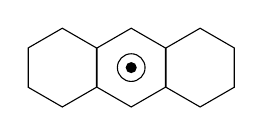
\begin{tikzpicture}
        \hexgrid{2}{0}
        \punit{0/0,2/0}{a}
        \pivot{1}{0}
    \end{tikzpicture}
    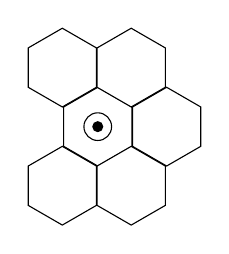
\begin{tikzpicture}
        \hexgrid{1}{2}
        \punit{1/0,0/0,0/2}{b}
        \pivot{0}{1}
    \end{tikzpicture}
    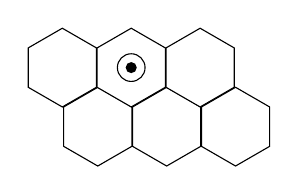
\begin{tikzpicture}
        \hexgrid{2}{1}
        \punit{2/0,1/0,0/1}{c}
        \pivot{1}{0}
    \end{tikzpicture}
    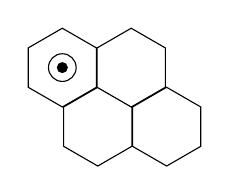
\begin{tikzpicture}
        \hexgrid{1}{1}
        \punit{1/1,1/0,0/1}{d}
        \pivot{0}{0}
    \end{tikzpicture}
    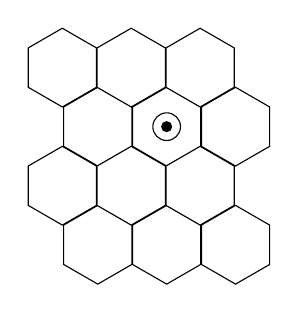
\begin{tikzpicture}
        \hexgrid{2}{3}
        \punit{2/0,1/1,1/2,0/3}{e}
        \pivot{1}{1}
    \end{tikzpicture}
    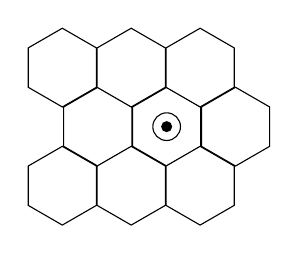
\begin{tikzpicture}
        \hexgrid{2}{2}
        \punit{2/0,1/0,0/1,0/2}{f}
        \pivot{1}{1}
    \end{tikzpicture}
    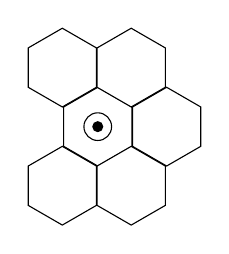
\begin{tikzpicture}
        \hexgrid{1}{2}
        \punit{1/1,1/0,0/1,0/2}{g}
        \pivot{0}{1}
    \end{tikzpicture}
    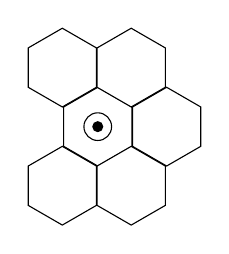
\begin{tikzpicture}
        \hexgrid{1}{2}
        \punit{0/0,1/0,0/1,0/2}{h}
        \pivot{0}{1}
    \end{tikzpicture}
    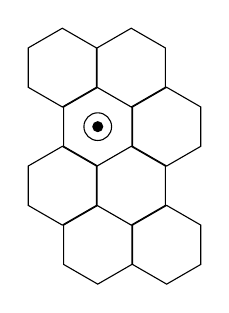
\begin{tikzpicture}
        \hexgrid{1}{3}
        \punit{1/0,1/1,1/2,0/3}{i}
        \pivot{0}{1}
    \end{tikzpicture}
    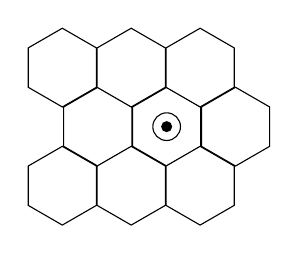
\begin{tikzpicture}
        \hexgrid{2}{2}
        \punit{2/0,1/1,0/1,0/2}{j}
        \pivot{1}{1}
    \end{tikzpicture}
    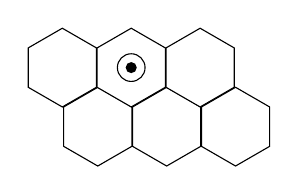
\begin{tikzpicture}
        \hexgrid{2}{1}
        \punit{2/1,2/0,1/0,0/1}{k}
        \pivot{1}{0}
    \end{tikzpicture}
    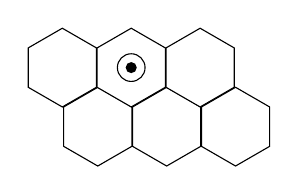
\begin{tikzpicture}
        \hexgrid{2}{1}
        \punit{1/1,2/0,1/0,0/1}{l}
        \pivot{1}{0}
    \end{tikzpicture}
    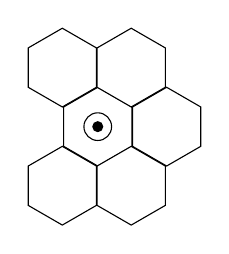
\begin{tikzpicture}
        \hexgrid{1}{2}
        \punit{0/0,0/1,1/1,0/2}{m}
        \pivot{0}{1}
    \end{tikzpicture}
    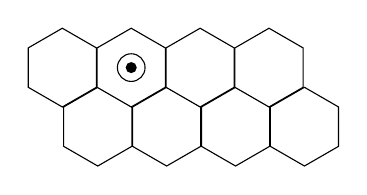
\begin{tikzpicture}
        \hexgrid{3}{1}
        \punit{0/1,1/1,3/0,2/0}{n}
        \pivot{1}{0}
    \end{tikzpicture}
\fi


        \item \ifdessins
\begin{tikzpicture}[scale=0.9,every node/.style={transform shape}]
\hexgrid{39}{19}\node[hexcell,piecei] at (h12;4.south) {};\node[hexcell,piecei] at (h13;4.south) {};\node[hexcell,piecek] at (h19;4.south) {};\node[hexcell,piecek] at (h23;4.south) {};\node[hexcell,piecek] at (h25;4.south) {};\node[hexcell,piecem] at (h26;4.south) {};\node[hexcell,pieceh] at (h28;4.south) {};\node[hexcell,piecec] at (h31;4.south) {};\node[hexcell,pieceg] at (h34;4.south) {};\node[hexcell,piecej] at (h38;4.south) {};\node[hexcell,piecee] at (h8;5.south) {};\node[hexcell,piecee] at (h9;5.south) {};\node[hexcell,piecee] at (h10;5.south) {};\node[hexcell,piecee] at (h11;5.south) {};\node[hexcell,piecei] at (h12;5.south) {};\node[hexcell,piecei] at (h13;5.south) {};\node[hexcell,piecek] at (h15;5.south) {};\node[hexcell,piecek] at (h16;5.south) {};\node[hexcell,piecek] at (h19;5.south) {};\node[hexcell,pieceh] at (h22;5.south) {};\node[hexcell,piecek] at (h23;5.south) {};\node[hexcell,piecek] at (h24;5.south) {};\node[hexcell,piecem] at (h25;5.south) {};\node[hexcell,piecem] at (h26;5.south) {};\node[hexcell,piecem] at (h27;5.south) {};\node[hexcell,pieceh] at (h28;5.south) {};\node[hexcell,pieceh] at (h29;5.south) {};\node[hexcell,piecec] at (h30;5.south) {};\node[hexcell,piecei] at (h31;5.south) {};\node[hexcell,pieceg] at (h33;5.south) {};\node[hexcell,pieceg] at (h34;5.south) {};\node[hexcell,piecej] at (h36;5.south) {};\node[hexcell,piecej] at (h37;5.south) {};\node[hexcell,filled] at (h0;6.south) {};\node[hexcell,filled] at (h4;6.south) {};\node[hexcell,piecec] at (h7;6.south) {};\node[hexcell,piecek] at (h8;6.south) {};\node[hexcell,piecek] at (h9;6.south) {};\node[hexcell,piecei] at (h10;6.south) {};\node[hexcell,piecei] at (h11;6.south) {};\node[hexcell,piecei] at (h12;6.south) {};\node[hexcell,pieced] at (h13;6.south) {};\node[hexcell,piecei] at (h14;6.south) {};\node[hexcell,piecek] at (h15;6.south) {};\node[hexcell,piecef] at (h17;6.south) {};\node[hexcell,piecek] at (h18;6.south) {};\node[hexcell,piecek] at (h19;6.south) {};\node[hexcell,piecen] at (h20;6.south) {};\node[hexcell,piecen] at (h21;6.south) {};\node[hexcell,pieceh] at (h22;6.south) {};\node[hexcell,piecek] at (h23;6.south) {};\node[hexcell,piecem] at (h24;6.south) {};\node[hexcell,piecem] at (h25;6.south) {};\node[hexcell,piecem] at (h26;6.south) {};\node[hexcell,pieceh] at (h27;6.south) {};\node[hexcell,pieceh] at (h28;6.south) {};\node[hexcell,pieceh] at (h29;6.south) {};\node[hexcell,filled] at (h30;6.south) {};\node[hexcell,piecec] at (h31;6.south) {};\node[hexcell,piecei] at (h32;6.south) {};\node[hexcell,pieceg] at (h33;6.south) {};\node[hexcell,filled] at (h34;6.south) {};\node[hexcell,piecek] at (h35;6.south) {};\node[hexcell,piecej] at (h36;6.south) {};\node[hexcell,piecek] at (h37;6.south) {};\node[hexcell,pieceg] at (h38;6.south) {};\node[hexcell,piecej] at (h39;6.south) {};\node[hexcell,filled] at (h1;7.south) {};\node[hexcell,filled] at (h4;7.south) {};\node[hexcell,piecec] at (h5;7.south) {};\node[hexcell,piecec] at (h6;7.south) {};\node[hexcell,piecee] at (h7;7.south) {};\node[hexcell,piecee] at (h8;7.south) {};\node[hexcell,piecek] at (h9;7.south) {};\node[hexcell,piecef] at (h10;7.south) {};\node[hexcell,piecei] at (h11;7.south) {};\node[hexcell,pieced] at (h12;7.south) {};\node[hexcell,pieced] at (h13;7.south) {};\node[hexcell,piecem] at (h14;7.south) {};\node[hexcell,piecek] at (h15;7.south) {};\node[hexcell,piecef] at (h16;7.south) {};\node[hexcell,piecee] at (h17;7.south) {};\node[hexcell,piecen] at (h18;7.south) {};\node[hexcell,piecen] at (h19;7.south) {};\node[hexcell,piecei] at (h20;7.south) {};\node[hexcell,pieceh] at (h21;7.south) {};\node[hexcell,pieceh] at (h22;7.south) {};\node[hexcell,piecek] at (h23;7.south) {};\node[hexcell,piecek] at (h24;7.south) {};\node[hexcell,piecem] at (h25;7.south) {};\node[hexcell,piecem] at (h26;7.south) {};\node[hexcell,pieceh] at (h27;7.south) {};\node[hexcell,piecef] at (h28;7.south) {};\node[hexcell,piecef] at (h29;7.south) {};\node[hexcell,filled] at (h30;7.south) {};\node[hexcell,pieceg] at (h31;7.south) {};\node[hexcell,piecei] at (h32;7.south) {};\node[hexcell,piecei] at (h33;7.south) {};\node[hexcell,filled] at (h34;7.south) {};\node[hexcell,piecek] at (h35;7.south) {};\node[hexcell,piecek] at (h36;7.south) {};\node[hexcell,pieceg] at (h37;7.south) {};\node[hexcell,pieceg] at (h38;7.south) {};\node[hexcell,piecej] at (h39;7.south) {};\node[hexcell,piecee] at (h0;8.south) {};\node[hexcell,filled] at (h1;8.south) {};\node[hexcell,filled] at (h3;8.south) {};\node[hexcell,piecel] at (h5;8.south) {};\node[hexcell,piecel] at (h6;8.south) {};\node[hexcell,piecee] at (h7;8.south) {};\node[hexcell,piecee] at (h8;8.south) {};\node[hexcell,piecek] at (h9;8.south) {};\node[hexcell,piecej] at (h10;8.south) {};\node[hexcell,piecef] at (h11;8.south) {};\node[hexcell,piecei] at (h12;8.south) {};\node[hexcell,piecem] at (h13;8.south) {};\node[hexcell,piecem] at (h14;8.south) {};\node[hexcell,piecef] at (h15;8.south) {};\node[hexcell,piecef] at (h16;8.south) {};\node[hexcell,piecee] at (h17;8.south) {};\node[hexcell,piecei] at (h18;8.south) {};\node[hexcell,piecei] at (h19;8.south) {};\node[hexcell,piecei] at (h20;8.south) {};\node[hexcell,piecem] at (h21;8.south) {};\node[hexcell,piecek] at (h22;8.south) {};\node[hexcell,piecek] at (h23;8.south) {};\node[hexcell,piecek] at (h24;8.south) {};\node[hexcell,piecem] at (h25;8.south) {};\node[hexcell,piecem] at (h26;8.south) {};\node[hexcell,pieceh] at (h27;8.south) {};\node[hexcell,piecef] at (h28;8.south) {};\node[hexcell,piecef] at (h29;8.south) {};\node[hexcell,filled] at (h30;8.south) {};\node[hexcell,pieceg] at (h31;8.south) {};\node[hexcell,pieceg] at (h32;8.south) {};\node[hexcell,pieceg] at (h33;8.south) {};\node[hexcell,filled] at (h34;8.south) {};\node[hexcell,pieceg] at (h36;8.south) {};\node[hexcell,pieceg] at (h37;8.south) {};\node[hexcell,piecek] at (h38;8.south) {};\node[hexcell,piecej] at (h39;8.south) {};\node[hexcell,piecee] at (h0;9.south) {};\node[hexcell,filled] at (h2;9.south) {};\node[hexcell,filled] at (h3;9.south) {};\node[hexcell,piecel] at (h4;9.south) {};\node[hexcell,piecel] at (h5;9.south) {};\node[hexcell,piecee] at (h6;9.south) {};\node[hexcell,piecee] at (h7;9.south) {};\node[hexcell,piecek] at (h8;9.south) {};\node[hexcell,piecek] at (h9;9.south) {};\node[hexcell,piecej] at (h10;9.south) {};\node[hexcell,piecef] at (h11;9.south) {};\node[hexcell,piecei] at (h12;9.south) {};\node[hexcell,piecei] at (h13;9.south) {};\node[hexcell,piecem] at (h14;9.south) {};\node[hexcell,piecee] at (h16;9.south) {};\node[hexcell,piecee] at (h17;9.south) {};\node[hexcell,piecee] at (h18;9.south) {};\node[hexcell,piecee] at (h19;9.south) {};\node[hexcell,piecee] at (h20;9.south) {};\node[hexcell,piecem] at (h21;9.south) {};\node[hexcell,piecem] at (h22;9.south) {};\node[hexcell,piecem] at (h23;9.south) {};\node[hexcell,piecek] at (h24;9.south) {};\node[hexcell,piecek] at (h25;9.south) {};\node[hexcell,piecem] at (h26;9.south) {};\node[hexcell,piecef] at (h27;9.south) {};\node[hexcell,piecef] at (h28;9.south) {};\node[hexcell,filled] at (h29;9.south) {};\node[hexcell,filled] at (h30;9.south) {};\node[hexcell,filled] at (h31;9.south) {};\node[hexcell,filled] at (h32;9.south) {};\node[hexcell,filled] at (h34;9.south) {};\node[hexcell,pieceg] at (h35;9.south) {};\node[hexcell,pieceg] at (h36;9.south) {};\node[hexcell,pieceg] at (h37;9.south) {};\node[hexcell,piecek] at (h38;9.south) {};\node[hexcell,piecej] at (h39;9.south) {};\node[hexcell,piecee] at (h1;10.south) {};\node[hexcell,filled] at (h2;10.south) {};\node[hexcell,filled] at (h5;10.south) {};\node[hexcell,piecee] at (h6;10.south) {};\node[hexcell,piecee] at (h7;10.south) {};\node[hexcell,piecek] at (h8;10.south) {};\node[hexcell,filled] at (h9;10.south) {};\node[hexcell,piecej] at (h10;10.south) {};\node[hexcell,piecef] at (h11;10.south) {};\node[hexcell,filled] at (h12;10.south) {};\node[hexcell,filled] at (h13;10.south) {};\node[hexcell,filled] at (h14;10.south) {};\node[hexcell,piecee] at (h16;10.south) {};\node[hexcell,pieced] at (h17;10.south) {};\node[hexcell,filled] at (h18;10.south) {};\node[hexcell,filled] at (h19;10.south) {};\node[hexcell,filled] at (h20;10.south) {};\node[hexcell,piecem] at (h21;10.south) {};\node[hexcell,piecem] at (h22;10.south) {};\node[hexcell,piecem] at (h23;10.south) {};\node[hexcell,filled] at (h24;10.south) {};\node[hexcell,filled] at (h25;10.south) {};\node[hexcell,filled] at (h26;10.south) {};\node[hexcell,piecef] at (h27;10.south) {};\node[hexcell,piecef] at (h28;10.south) {};\node[hexcell,filled] at (h30;10.south) {};\node[hexcell,filled] at (h34;10.south) {};\node[hexcell,filled] at (h35;10.south) {};\node[hexcell,filled] at (h36;10.south) {};\node[hexcell,piecek] at (h37;10.south) {};\node[hexcell,piecek] at (h38;10.south) {};\node[hexcell,piecem] at (h39;10.south) {};\node[hexcell,piecee] at (h1;11.south) {};\node[hexcell,filled] at (h2;11.south) {};\node[hexcell,filled] at (h6;11.south) {};\node[hexcell,piecem] at (h7;11.south) {};\node[hexcell,piecek] at (h8;11.south) {};\node[hexcell,filled] at (h9;11.south) {};\node[hexcell,piecej] at (h10;11.south) {};\node[hexcell,filled] at (h12;11.south) {};\node[hexcell,filled] at (h15;11.south) {};\node[hexcell,pieced] at (h16;11.south) {};\node[hexcell,pieced] at (h17;11.south) {};\node[hexcell,filled] at (h18;11.south) {};\node[hexcell,filled] at (h21;11.south) {};\node[hexcell,piecem] at (h23;11.south) {};\node[hexcell,filled] at (h24;11.south) {};\node[hexcell,filled] at (h27;11.south) {};\node[hexcell,piecel] at (h28;11.south) {};\node[hexcell,piecel] at (h29;11.south) {};\node[hexcell,filled] at (h30;11.south) {};\node[hexcell,filled] at (h34;11.south) {};\node[hexcell,filled] at (h37;11.south) {};\node[hexcell,piecem] at (h38;11.south) {};\node[hexcell,piecem] at (h39;11.south) {};\node[hexcell,filled] at (h2;12.south) {};\node[hexcell,filled] at (h5;12.south) {};\node[hexcell,piecem] at (h7;12.south) {};\node[hexcell,piecem] at (h8;12.south) {};\node[hexcell,filled] at (h9;12.south) {};\node[hexcell,filled] at (h11;12.south) {};\node[hexcell,filled] at (h15;12.south) {};\node[hexcell,filled] at (h17;12.south) {};\node[hexcell,filled] at (h21;12.south) {};\node[hexcell,filled] at (h23;12.south) {};\node[hexcell,filled] at (h27;12.south) {};\node[hexcell,piecel] at (h28;12.south) {};\node[hexcell,piecel] at (h29;12.south) {};\node[hexcell,filled] at (h30;12.south) {};\node[hexcell,filled] at (h34;12.south) {};\node[hexcell,filled] at (h37;12.south) {};\node[hexcell,piecem] at (h39;12.south) {};\node[hexcell,filled] at (h2;13.south) {};\node[hexcell,filled] at (h6;13.south) {};\node[hexcell,piecem] at (h7;13.south) {};\node[hexcell,filled] at (h9;13.south) {};\node[hexcell,filled] at (h12;13.south) {};\node[hexcell,filled] at (h15;13.south) {};\node[hexcell,filled] at (h18;13.south) {};\node[hexcell,filled] at (h21;13.south) {};\node[hexcell,filled] at (h24;13.south) {};\node[hexcell,filled] at (h27;13.south) {};\node[hexcell,pieceh] at (h28;13.south) {};\node[hexcell,filled] at (h30;13.south) {};\node[hexcell,filled] at (h34;13.south) {};\node[hexcell,filled] at (h37;13.south) {};\node[hexcell,filled] at (h2;14.south) {};\node[hexcell,filled] at (h6;14.south) {};\node[hexcell,filled] at (h7;14.south) {};\node[hexcell,filled] at (h8;14.south) {};\node[hexcell,filled] at (h12;14.south) {};\node[hexcell,filled] at (h13;14.south) {};\node[hexcell,filled] at (h14;14.south) {};\node[hexcell,filled] at (h15;14.south) {};\node[hexcell,filled] at (h18;14.south) {};\node[hexcell,filled] at (h19;14.south) {};\node[hexcell,filled] at (h20;14.south) {};\node[hexcell,filled] at (h21;14.south) {};\node[hexcell,filled] at (h24;14.south) {};\node[hexcell,filled] at (h25;14.south) {};\node[hexcell,filled] at (h26;14.south) {};\node[hexcell,pieceh] at (h28;14.south) {};\node[hexcell,filled] at (h30;14.south) {};\node[hexcell,filled] at (h31;14.south) {};\node[hexcell,filled] at (h34;14.south) {};\node[hexcell,filled] at (h37;14.south) {};\node[hexcell,piecen] at (h0;15.south) {};\node[hexcell,filled] at (h15;15.south) {};\node[hexcell,filled] at (h21;15.south) {};\node[hexcell,pieceh] at (h25;15.south) {};\node[hexcell,piecec] at (h26;15.south) {};\node[hexcell,pieceh] at (h27;15.south) {};\node[hexcell,pieceh] at (h28;15.south) {};\node[hexcell,piecel] at (h29;15.south) {};\node[hexcell,piecel] at (h30;15.south) {};\node[hexcell,piecen] at (h0;16.south) {};\node[hexcell,piecea] at (h1;16.south) {};\node[hexcell,piecea] at (h3;16.south) {};\node[hexcell,pieceb] at (h4;16.south) {};\node[hexcell,pieceb] at (h5;16.south) {};\node[hexcell,pieceb] at (h6;16.south) {};\node[hexcell,piecea] at (h7;16.south) {};\node[hexcell,filled] at (h14;16.south) {};\node[hexcell,piecea] at (h19;16.south) {};\node[hexcell,filled] at (h20;16.south) {};\node[hexcell,piecea] at (h21;16.south) {};\node[hexcell,piecel] at (h22;16.south) {};\node[hexcell,piecel] at (h23;16.south) {};\node[hexcell,pieceh] at (h24;16.south) {};\node[hexcell,pieceh] at (h25;16.south) {};\node[hexcell,pieceh] at (h26;16.south) {};\node[hexcell,piecec] at (h27;16.south) {};\node[hexcell,piecec] at (h28;16.south) {};\node[hexcell,piecel] at (h29;16.south) {};\node[hexcell,piecel] at (h30;16.south) {};\node[hexcell,piecea] at (h31;16.south) {};\node[hexcell,pieced] at (h32;16.south) {};\node[hexcell,piecea] at (h33;16.south) {};\node[hexcell,piecel] at (h34;16.south) {};\node[hexcell,piecel] at (h35;16.south) {};\node[hexcell,pieceb] at (h37;16.south) {};\node[hexcell,piecen] at (h0;17.south) {};\node[hexcell,piecea] at (h1;17.south) {};\node[hexcell,pieceb] at (h2;17.south) {};\node[hexcell,pieceb] at (h3;17.south) {};\node[hexcell,pieceb] at (h4;17.south) {};\node[hexcell,pieceb] at (h5;17.south) {};\node[hexcell,pieceb] at (h6;17.south) {};\node[hexcell,pieceb] at (h7;17.south) {};\node[hexcell,pieceb] at (h8;17.south) {};\node[hexcell,pieceb] at (h9;17.south) {};\node[hexcell,pieceb] at (h10;17.south) {};\node[hexcell,filled] at (h12;17.south) {};\node[hexcell,filled] at (h13;17.south) {};\node[hexcell,filled] at (h14;17.south) {};\node[hexcell,filled] at (h18;17.south) {};\node[hexcell,filled] at (h19;17.south) {};\node[hexcell,filled] at (h20;17.south) {};\node[hexcell,piecel] at (h21;17.south) {};\node[hexcell,piecel] at (h22;17.south) {};\node[hexcell,piecej] at (h23;17.south) {};\node[hexcell,piecej] at (h24;17.south) {};\node[hexcell,pieceg] at (h25;17.south) {};\node[hexcell,pieceg] at (h26;17.south) {};\node[hexcell,pieceg] at (h27;17.south) {};\node[hexcell,piecef] at (h28;17.south) {};\node[hexcell,piecef] at (h29;17.south) {};\node[hexcell,piecef] at (h30;17.south) {};\node[hexcell,pieced] at (h31;17.south) {};\node[hexcell,pieced] at (h32;17.south) {};\node[hexcell,piecel] at (h33;17.south) {};\node[hexcell,piecel] at (h34;17.south) {};\node[hexcell,pieced] at (h35;17.south) {};\node[hexcell,pieced] at (h36;17.south) {};\node[hexcell,pieceb] at (h37;17.south) {};\node[hexcell,piecen] at (h0;18.south) {};\node[hexcell,piecel] at (h2;18.south) {};\node[hexcell,piecel] at (h3;18.south) {};\node[hexcell,pieced] at (h4;18.south) {};\node[hexcell,pieced] at (h5;18.south) {};\node[hexcell,piecea] at (h6;18.south) {};\node[hexcell,pieced] at (h7;18.south) {};\node[hexcell,pieced] at (h8;18.south) {};\node[hexcell,pieceb] at (h9;18.south) {};\node[hexcell,pieceb] at (h10;18.south) {};\node[hexcell,pieceb] at (h11;18.south) {};\node[hexcell,piecea] at (h21;18.south) {};\node[hexcell,piecei] at (h22;18.south) {};\node[hexcell,piecea] at (h23;18.south) {};\node[hexcell,pieceh] at (h24;18.south) {};\node[hexcell,piecej] at (h25;18.south) {};\node[hexcell,piecej] at (h26;18.south) {};\node[hexcell,pieceg] at (h27;18.south) {};\node[hexcell,piecef] at (h28;18.south) {};\node[hexcell,piecef] at (h29;18.south) {};\node[hexcell,piecef] at (h30;18.south) {};\node[hexcell,piecef] at (h31;18.south) {};\node[hexcell,pieceg] at (h32;18.south) {};\node[hexcell,pieceb] at (h33;18.south) {};\node[hexcell,pieceb] at (h34;18.south) {};\node[hexcell,pieceb] at (h35;18.south) {};\node[hexcell,pieced] at (h36;18.south) {};\node[hexcell,piecei] at (h37;18.south) {};\node[hexcell,pieceb] at (h38;18.south) {};\node[hexcell,piecea] at (h39;18.south) {};\node[hexcell,piecea] at (h0;19.south) {};\node[hexcell,pieceg] at (h1;19.south) {};\node[hexcell,piecel] at (h2;19.south) {};\node[hexcell,piecel] at (h3;19.south) {};\node[hexcell,pieceg] at (h4;19.south) {};\node[hexcell,pieced] at (h5;19.south) {};\node[hexcell,piecel] at (h6;19.south) {};\node[hexcell,piecel] at (h7;19.south) {};\node[hexcell,pieced] at (h8;19.south) {};\node[hexcell,pieced] at (h9;19.south) {};\node[hexcell,piecel] at (h10;19.south) {};\node[hexcell,piecel] at (h11;19.south) {};\node[hexcell,pieceh] at (h14;19.south) {};\node[hexcell,pieceh] at (h15;19.south) {};\node[hexcell,pieceh] at (h16;19.south) {};\node[hexcell,pieceh] at (h17;19.south) {};\node[hexcell,piecei] at (h19;19.south) {};\node[hexcell,piecei] at (h20;19.south) {};\node[hexcell,piecei] at (h21;19.south) {};\node[hexcell,piecei] at (h22;19.south) {};\node[hexcell,pieceh] at (h23;19.south) {};\node[hexcell,pieceh] at (h24;19.south) {};\node[hexcell,pieceh] at (h25;19.south) {};\node[hexcell,piecek] at (h26;19.south) {};\node[hexcell,piecea] at (h27;19.south) {};\node[hexcell,piecek] at (h28;19.south) {};\node[hexcell,piecea] at (h29;19.south) {};\node[hexcell,piecef] at (h30;19.south) {};\node[hexcell,pieceg] at (h31;19.south) {};\node[hexcell,pieceg] at (h32;19.south) {};\node[hexcell,pieceg] at (h33;19.south) {};\node[hexcell,piecei] at (h34;19.south) {};\node[hexcell,piecei] at (h35;19.south) {};\node[hexcell,piecei] at (h36;19.south) {};\node[hexcell,pieceb] at (h37;19.south) {};\node[hexcell,pieceb] at (h38;19.south) {};\node[hexcell,pieceb] at (h39;19.south) {};%% END Step 18
\end{tikzpicture}
\fi

\end{enumerate}
\end{figure}


\subsection{Encodage d'une solution}
Une solution � une partie est une cha�ne de caract�res encodant la suite de mouvements �
effectuer o� chaque mouvement peut �tre encod� par plusieurs caract�res selon la correspondance 
pr�sent�e dans la figure~\ref{fig:moves}.
\begin{figure}
    \caption{\label{fig:moves}Correspondance entre les mouvements et les caract�res}
    \centering
\begin{tabular}{r|l}
    mouvement & caract�res \\
    \hline
    $\sW$ & {\tt p'!.03} \\
    $\sE$ & {\tt bcefy2} \\
    $\sSW$ & {\tt aghij4} \\
    $\sSE$ & {\tt lmno 5} \\
    $\sCW$ & {\tt dqrvz1} \\
    $\sCCW$ & {\tt kstuwx}
\end{tabular}
\end{figure}

\subsection{Phrases sp�ciales}
Dans la mesure o� il est possible d'utiliser plusieurs caract�res pour encoder un mouvement,
une m�me solution peut s'exprimer d'un grand nombre de mani�res, certaines d'entre elles faisant
appara�tre des mots compr�hensibles.

Une part importante du score final pour une partie est d�termin� par la fr�quence d'apparition 
de phrases sp�ciales d�crites � la figure~\ref{fig:power}.

On peut remarquer que certaines de ces phrases sont longues et n�cessitent beaucoup de cases
libres pour �tre jou�es sans coups invalides. Lorsqu'une pi�ce a certaines sym�tries de rotation 
vis-�-vis de son pivot, elles peuvent �tre toujours invalides. Par exemple pour une pi�ce triviale
r�duite � une seule case contenant son pivot aucune des phrases contenant des rotations n'est 
valide.

Lors des trois jours du concours les phrases sp�ciales �taient cach�es, pour les obtenir il 
fallait r�soudre des devinettes apparaissant au fil du d�roulement. Notre �quipe a d�couvert 15 
des 18 phrases sp�ciales\footnote{Dont 5 dans la derni�re heure gr�ce � des �changes avec 
d'autres �quipes\dots}.

\begin{figure}
    \caption{\label{fig:power}Les diff�rentes phrases sp�ciales, num�rot�es de
    1 � 18, et leurs mouvements associ�s}
    \centering
    \small

    \begin{description}
        \item[1 {\tt in his house at r'lyeh dead cthulhu waits dreaming.}]
            $\sSW\sSE\sSE\sSW\sSW\sCCW\sSE\sSW\sSE\sCCW\sCCW\sE\sSE\sSW\sCCW\sSE$ \\ $\sCW\sW\sSE\sE\sE\sSW\sSE\sCW\sE\sSW\sCW\sSE\sE\sCCW\sSW\sCCW\sSE\sSW\sCCW\sSE\sCCW\sSW\sSW\sCCW\sCCW\sSE\sCW\sCW\sE\sSW\sSE\sSW\sSE\sSW\sW$
    \item[2 {\tt ph'nglui mglw'nafh cthulhu r'lyeh wgah'nagl fhtagn.}] 
            $\sW\sSW\sW\sSE\sSW\sSE\sCCW\sSW\sSE\sSE\sSW\sSE\sCCW\sW\sSE\sSW\sE$ \\ $\sSW\sSE\sE\sCCW\sSW\sCCW\sSE\sSW\sCCW\sSE\sCW\sW\sSE\sE\sE\sSW\sSE\sCCW\sSW\sSW\sSW\sW\sSE\sSW\sSW\sSE\sSE\sE\sSW\sCCW\sSW\sSW\sSE\sW$

    \item[3 {\tt case nightmare green}] $\sE\sSW\sCCW\sE\sSE\sSE\sSW\sSW\sSW\sCCW\sSE\sSW\sCW\sE\sSE\sSW\sCW\sE\sE\sSE$
    \item[4 {\tt cthulhu fhtagn!}] $\sE\sCCW\sSW\sCCW\sSE\sSW\sCCW\sSE\sE\sSW\sCCW\sSW\sSW\sSE\sW$
    \item[5 {\tt john bigboote}] $\sSW\sSE\sSW\sSE\sSE\sE\sSW\sSW\sE\sSE\sSE\sCCW\sE$ 
    \item[6 {\tt vigintillion}] $\sCW\sSW\sSW\sSW\sSE\sCCW\sSW\sSE\sSE\sSW\sSE\sSE$ 
    \item[7 {\tt necronomicon}] $\sSE\sE\sE\sCW\sSE\sSE\sSE\sSE\sSW\sE\sSE\sSE$
    \item[8 {\tt the laundry}] $\sCCW\sSW\sE\sSE\sSE\sSW\sCCW\sSE\sCW\sCW\sE$
    \item[9 {\tt yogsothoth}] $\sE\sSE\sSW\sCCW\sSE\sCCW\sSW\sSE\sCCW\sSW$
    \item[10 {\tt blue hades}] $\sE\sSE\sCCW\sE\sSE\sSW\sSW\sCW\sE\sCCW$
    \item[11 {\tt tsathoggua}] $\sCCW\sCCW\sSW\sCCW\sSW\sSE\sSW\sSW\sCCW\sSW$
    \item[12 {\tt monkeyboy}] $\sSE\sSE\sSE\sCCW\sE\sE\sE\sSE\sE$
    \item[13 {\tt planet 10}] $\sW\sSE\sSW\sSE\sE\sCCW\sSE\sCW\sW$
    \item[14 {\tt yoyodyne}] $\sE\sSE\sE\sSE\sCW\sE\sSE\sE$
    \item[15 {\tt ia! ia!}] $\sSW\sSW\sW\sSE\sSW\sSW\sW$
    \item[16 {\tt yuggoth}] $\sE\sCCW\sSW\sSW\sSE\sCCW\sSW$
    \item[17 {\tt r'lyeh}] $\sCW\sW\sSE\sE\sE\sSW$
    \item[18 {\tt ei!}] $\sE\sSW\sW$
\end{description}
\end{figure}

\subsection{R�p�tition de positions}
\label{par:stuttering}
Pour ne pas qu'on puisse exploiter les phrases sp�ciales en cr�ant des suites
de mouvements tr�s longues, il faut borner la longueur d'une suite de
mouvements.

Le plus simple pour cela est d'interdire de revenir dans une configuration
pr�c�dente du plateau. Comme le plateau change apr�s chaque verrouillage, il
est possible de simplifier la contrainte en interdisant qu'au cours de la suite
de mouvements d'une pi�ce donn�e celle-ci occupe une position pr�c�demment
emprunt�e.

Pour tenir compte des rotations, il faut �tre plus pr�cis. Deux positions
d'une pi�ce sont dites visuellement identiques quand :
\begin{itemize}
    \item le pivot est � la m�me position dans la grille ;
    \item toute cellule occup�e par une des pi�ces est occup�e par l'autre.
\end{itemize}

On interdit alors d'avoir deux positions visuellement identiques au cours d'un
mouvement.

C'est en consid�rant des pi�ces ayant des sym�tries de rotation que cette
condition prend tout son sens et montre qu'il ne s'agit pas uniquement
d'interdire les retours en arri�re. La figure~\ref{fig:stuttering} pr�sente un
exemple de suite de mouvements faisant apparaitre des positions visuellement
identiques.

\begin{figure}
    \caption{\label{fig:stuttering} Une suite de mouvement invalide car la
    premi�re et la derni�re position sont visuellement identiques}
    \centering
\ifdessins
    \[
\begin{tikzpicture}
\hexgrid{3}{2}
\node[hexcell,pieceo] at (h0;1.south) {};
\node[hexcell,pieceo] at (h2;0.south) {};
\node[hexcell,pieceo] at (h2;2.south) {};
\pivot{1}{1}
\mCW{1}{1}
\end{tikzpicture} 
\quad
\begin{tikzpicture}
\hexgrid{3}{2}
\node[hexcell,pieceo] at (h2;1.south) {};
\node[hexcell,pieceo] at (h1;0.south) {};
\node[hexcell,pieceo] at (h1;2.south) {};
\pivot{1}{1}
\mE{1}{1}
\end{tikzpicture}
\quad
\begin{tikzpicture}
\hexgrid{3}{2}
\node[hexcell,pieceo] at (h3;1.south) {};
\node[hexcell,pieceo] at (h2;0.south) {};
\node[hexcell,pieceo] at (h2;2.south) {};
\pivot{2}{1}
\mCW{2}{1}
\end{tikzpicture}
\quad
\begin{tikzpicture}
\hexgrid{3}{2}
\node[hexcell,pieceo] at (h1;1.south) {};
\node[hexcell,pieceo] at (h3;0.south) {};
\node[hexcell,pieceo] at (h3;2.south) {};
\pivot{2}{1}
\mW{2}{1}
\end{tikzpicture} 
\quad
\begin{tikzpicture}
\hexgrid{3}{2}
\node[hexcell,pieceo] at (h0;1.south) {};
\node[hexcell,pieceo] at (h2;0.south) {};
\node[hexcell,pieceo] at (h2;2.south) {};
\pivot{1}{1}
\end{tikzpicture} 
\]
\fi
\end{figure}


\section{Solution choisie}
\subsection{Syst�me de coordonn�es obliques et rotations}
Il existe un syst�me de coordonn�es g�om�triques simple pour une grille
hexagonale : \emph{le syst�me de coordonn�es obliques} qui est pr�sent� 
� la figure~\ref{fig:hexcoord2}.

Ce syst�me correspond aux coordonn�es dans la base
$(\vec{u},\vec{v}) = \left((1,0), (\frac{1}{2},-\frac{\sqrt{3}}{2})\right)$ 
de $\R^2$ pour des hexagones de diam�tre 1.
\iffalse
comme on peut le constater avec de la g�om�trie �l�mentaire pour la seule
coordonn�e posant probl�me :
\begin{center}
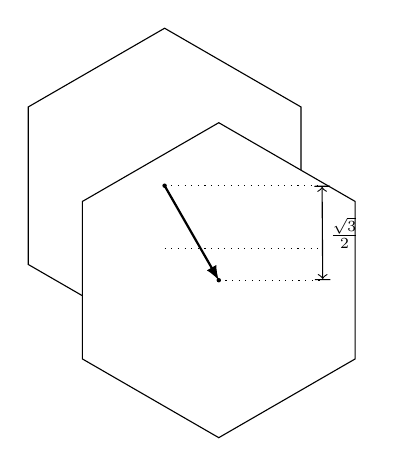
\begin{tikzpicture}[scale=4, every node/.style={transform shape}]
    \node[hexgrid]
        (h00) at (0.4*1.75*0*0.5+0.4*0.45*0,0.4*-1.5*0*0.5) {};
    \node[hexgrid]
        (h01) at (0.4*1.75*0*0.5+0.4*0.43*1,0.4*-1.5*1*0.5) {};

    \fill[black] (h00.center) circle (0.2pt);
    \fill[black] (h01.center) circle (0.2pt);
    \draw[-latex,thick] (h00.center) -- (h01.center);
    \coordinate (s0) at ($(h00.center) + (0.5,0)$);
    \coordinate (q1) at ($(h00.center) + (0,-0.2)$);
    \coordinate (s1) at ($(h00.center) + (0.5,-0.2)$);
    \coordinate (s2) at ($(h01.center) + (0.5-0.17,0)$);
    \draw[dotted] (q1) -- (s1);
    \draw[dotted] (h00.center) -- (s0);
    \draw[dotted] (h01.center) -- (s2);
    \draw[|<->|] (s0) -- node[scale=0.2,right] {$\frac{\sqrt{3}}{2}$} (s2);
\end{tikzpicture}
\end{center}
\fi
Pour passer du syst�me originel vers celui-ci il suffit d'appliquer la 
transformation
\[
(x,y) \xrightarrow{\text{vers oblique}} \left(x+\left\lfloor
\frac{y}{2}\right\rfloor, y\right)
\]
et pour revenir dans le syst�me originel il suffit de faire la r�ciproque
dans la mesure o� la seconde coordonn�e est inchang�e 
\[
(x,y) \xrightarrow{\text{vers originel}} \left(x-\left\lfloor
\frac{y}{2}\right\rfloor, y\right)
\]

L'avantage de ce syst�me est imm�diat quand on consid�re l'impact des
mouvements de descente sur les coordonn�es comme pr�sent� � la 
figure~\ref{fig:mouvement_systeme}.

Mais l� o� ce syst�me est particuli�rement int�ressant c'est qu'il permet
d'effectuer des rotations d'angle $\frac{k\pi}{3}$, $k \in \Z$, en utilisant
uniquement des op�rations arithm�tiques enti�res~\footnote{On pourrait objecter
que le passage d'un syst�me de coordonn�es � l'autre n�cessite une division,
mais comme il s'agit d'une division par deux, un simple d�calage � droite 
l'effectue, cette derni�re op�ration �tant encore plus �l�mentaire qu'une
addition.}.

Partant d'un point de coordonn�es $(x,y)$ dans la base canonique de $\R^2$, on
sait qu'en effectuant une rotation de centre l'origine et d'angle
$\frac{-\pi}{3}$ on aboutit au point de coordonn�es  $(x',y')$ o�
\[
x' = \frac{x + \sqrt{3}y}{2} \quad y' = \frac{-\sqrt{3}x + y}{2}
\]
On consid�re maintenant le point de coordonn�es obliques $(x_o,y_o)$
qui a donc pour coordonn�s dans $\R^2$ le couple 
$(x_o+\frac{y_o}{2}, - \frac{\sqrt{3}}{2} y_o)$. Apr�s rotation, on 
obtient le couple 
\[
\left(\frac{x_o + \frac{y_o}{2} - \sqrt{3}\frac{\sqrt{3}}{2}y_o}{2},
 \frac{-\sqrt{3}x_o - \frac{\sqrt{3}y_o}{2} - \frac{\sqrt{3}}{2} y_o}{2}\right)
 = \left(\frac{x_o}{2} - \frac{y_o}{2}, \frac{-\sqrt{3}}{2}(x_o + y_o) \right)
 = -y_o \vec{u} + (x_o+y_o)\vec{v}
\]
Pour effectuer un mouvement de rotation horaire dans le syst�me oblique on 
obtient ainsi la transformation �l�mentaire :
\[
    (x,y) \xrightarrow{\sCW} (-y,x+y)
\]
et en proc�dant de m�me on obtient 
\[
    (x,y) \xrightarrow{\sCCW} (x+y,-x)
\]
Notons qu'il est possible d'en d�duire une formule de rotation dans le syst�me
originel, ce qui donne pour la rotation horaire :
\begin{multline*}
    (x,y) \xrightarrow{\text{vers oblique}}
        \left( x + \left\lfloor \frac{y}{2} \right\rfloor, y \right)
    \xrightarrow{\sCW} 
        \left( -y,  x + \left\lfloor \frac{y}{2} \right\rfloor + y \right) \\
    \xrightarrow{\text{vers originel}}
    \left( -y +  
    \left\lfloor\frac{x + \left\lfloor \frac{y}{2} \right\rfloor + y}{2}\right\rfloor
    ,  x + \left\lfloor \frac{y}{2} \right\rfloor + y \right)
\end{multline*}

\begin{figure}
    \caption{\label{fig:hexcoord2}Syst�me de coordonn�es obliquess}
\ifdessins
\centering
\begin{tikzpicture}[scale=2, every node/.style={transform shape}]
    \hexgridoblique{4}{4}
    \foreach \x in {0,...,4} {
    \foreach \y in {0,...,4} {
        \node at (h\x;\y.center) {\tiny \x,\y};
    }
    }
\end{tikzpicture}
\fi
\end{figure}

\begin{figure}
    \caption{\label{fig:mouvement_systeme}Effet d'un mouvement sur les
    coordonn�es $(x,y)$ selon le syst�me de coordonn�es}
    \centering
\begin{tabular}{c||c|c}
    Mouvement & Coordonn�es probl�me & Coordonn�es obliques \\
    \hline
    \hline
    $\sW$ & $(x-1,y)$ & $(x-1,y)$ \\
    \hline
    $\sE$ & $(x+1,y)$ & $(x+1,y)$ \\
    \hline
    $\sSW$ & $\begin{cases} (x-1,y+1) & \text{ si } y \text{ pair} \\ (x,y+1) &
        \text{ sinon} \end{cases}$ & $(x-1,y+1)$ \\
    \hline
    $\sSE$ & $\begin{cases} (x,y+1) & \text{ si } y \text{ pair} \\ (x+1,y+1) &
        \text{ sinon} \end{cases}$ & $(x,y+1)$
\end{tabular}
\end{figure}

On peut alors choisir d'utiliser ces coordonn�es uniquement pour calculer les
positions apr�s transformation ou les utiliser partout en ne revenant aux
coordonn�es initiales que pour acc�der au plateau. Lors du concours nous avons
fait le premier choix car le code avec d�j� �t� �crit sans les rotations qui
sont arriv�es trop tard pour partir sur le bon syst�me de coordonn�es.

Notons un autre avantage du syst�me de coordonn�es obliques : la translation
est g�om�trique, donc un simple ajout aux coordonn�es.
Cela donne la possibilit� d'identifier une pi�ce � la position de son pivot et 
de sa rotation  tout en pouvant calculer tr�s simplement la position de ses cellules.
En effet, on peut calculer toutes les rotations d'une pi�ce au d�part
puis se contenter de translater les cellules.

\subsection{Identification unique des positions}
\label{par:id_unique}
Afin de pouvoir assurer qu'aucune r�p�tition de position a lieu il ne suffit pas de prendre 
en compte des couples $(M,r)$ o� $M$ est la position du pivot et $r$ la rotation effectu�s sur la 
pi�ce.

En effet, certaines pi�ces sont invariantes par certaines rotations et la seule donn�e de $r$
ne permet pas de le prendre en compte. On consid�re pour cela son groupe d'invariants.

Soit $p$ une pi�ce on note $r_p$ la rotation d'un angle $\frac{\pi}{6}$ autour de son pivot.

On note $R(p)$ le sous-groupe des isom�tries du plan engendr�es par $r_p$ et $I(p)$ 
le sous-groupe de $R(p)$ constitu� des �l�ments laissant $p$ invariante.

Pour une position donn�e du pivot, on a donc autant de possibilit�s pour la pi�ce que
d'�l�ments dans $G_r(p) = R(p) / I(p)$ (tous ces groupes sont ab�liens). 

Comme $R(p) \sim \Z/6\Z$ on a quatre cas pour $G_r(p)$ qui sont illustr�s dans la figure~\ref{fig:cassym}.

\begin{figure}
    \caption{\label{fig:cassym}Les quatre cas pour le groupe $G_r(p)$}
    \centering
        \begin{tabular}{c|l}
        $G_r(p)\sim \Z/k\Z$ & Exemple \\ \hline
        $k=6$ & 
\ifdessins
    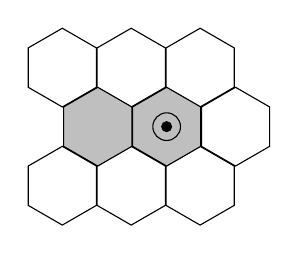
\begin{tikzpicture}
        \hexgrid{2}{2}
        \unit{0/1,1/1}
        \pivot{1}{1}
    \end{tikzpicture}
    {\Large $\circlearrowright$}
    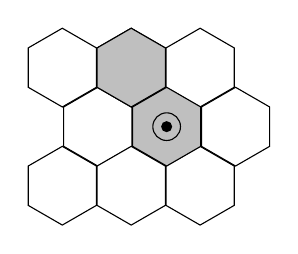
\begin{tikzpicture}
        \hexgrid{2}{2}
        \unit{1/0,1/1}
        \pivot{1}{1}
    \end{tikzpicture}
    {\Large $\circlearrowright$}
    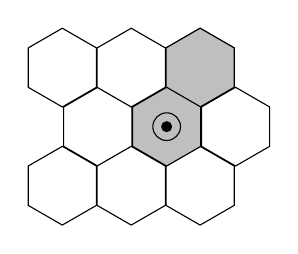
\begin{tikzpicture}
        \hexgrid{2}{2}
        \unit{2/0,1/1}
        \pivot{1}{1}
    \end{tikzpicture}
    {\Large $\circlearrowright$}
    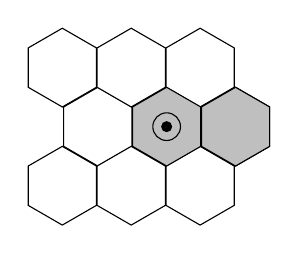
\begin{tikzpicture}
        \hexgrid{2}{2}
        \unit{2/1,1/1}
        \pivot{1}{1}
    \end{tikzpicture}
    {\Large $\circlearrowright$}
    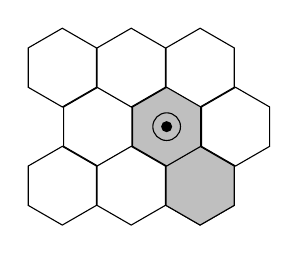
\begin{tikzpicture}
        \hexgrid{2}{2}
        \unit{2/2,1/1}
        \pivot{1}{1}
    \end{tikzpicture}
    {\Large $\circlearrowright$}
    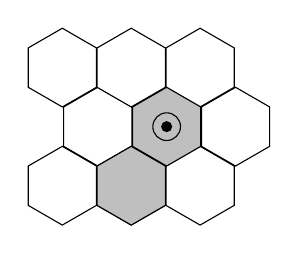
\begin{tikzpicture}
        \hexgrid{2}{2}
        \unit{1/2,1/1}
        \pivot{1}{1}
    \end{tikzpicture}
\fi
    \\
$k=3$ &
\ifdessins
    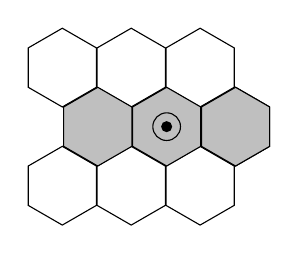
\begin{tikzpicture}
        \hexgrid{2}{2}
        \unit{0/1,1/1,2/1}
        \pivot{1}{1}
    \end{tikzpicture}
    {\Large $\circlearrowright$}
    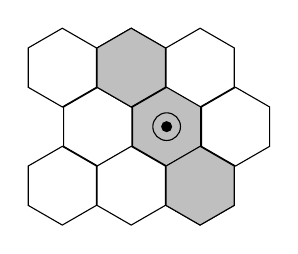
\begin{tikzpicture}
        \hexgrid{2}{2}
        \unit{1/0,1/1,2/2}
        \pivot{1}{1}
    \end{tikzpicture}
    {\Large $\circlearrowright$}
    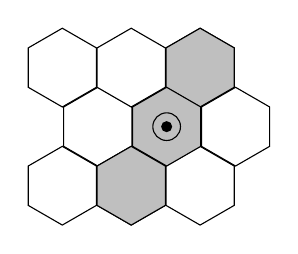
\begin{tikzpicture}
        \hexgrid{2}{2}
        \unit{2/0,1/1,1/2}
        \pivot{1}{1}
    \end{tikzpicture}
\fi
\\
$k=2$ & 
\ifdessins
    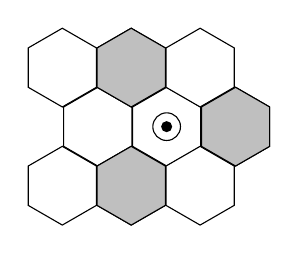
\begin{tikzpicture}
        \hexgrid{2}{2}
        \unit{1/0,2/1,1/2}
        \pivot{1}{1}
    \end{tikzpicture}
    {\Large $\circlearrowright$}
    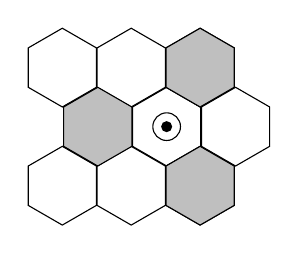
\begin{tikzpicture}
        \hexgrid{2}{2}
        \unit{0/1,2/0,2/2}
        \pivot{1}{1}
    \end{tikzpicture}
\fi
\\
$k=1$ & 
\ifdessins
    \begin{tikzpicture}
        \hexcell{0}{0}
        \pivot{0}{0}
    \end{tikzpicture} ,
    \begin{tikzpicture}
        \hexgrid{2}{2}
        \unit{1/0,2/0,0/1,1/1,2/1,1/2,2/2}
        \pivot{1}{1}
    \end{tikzpicture} 
\fi
\end{tabular}

\end{figure}

On peut alors repr�senter uniquement la position d'une pi�ce � sym�trie pr�s par un couple 
$(M,r)$ o� $M$ est la position du pivot et $r \in G_r(p)$.

En pratique, on identifie $r$ � l'�l�ment $k \in [|0;5|]$ tel que $r$ soit 
associ� � $\overline{k}$ par les isomorphismes ci-dessus.

On est donc ramen� � un triplet d'entier par position. Comme le pivot peut sortir
de la zone de jeu, il faut border le tableau pour pouvoir tenir compte de ces positions du pivot.

Un calcul rapide sur les pi�ces disponibles permet de d�terminer une valeur $b$ telle que le pivot 
dans une zone de jeu de dimension $w \times h$ ait des coordonn�es dans $[|-b;w+b-1|] \times
[|-b;h+b-1|]$. 

Gr�ce � cet encodage on peut cr�er un tableau de bool�ens � trois dimensions $V$ tel que 
$V_{x,y,k}$ indique si la position o� le pivot est en $(x,y)$ et la rotation est celle associ�e 
� $k$ est visit�e.~\footnote{Durant le concours, en raison de la pr�sence du bord $b$ � calculer 
et des probl�mes potentiels, nous avons uniquement utilis� une liste de positions visit�es ce 
qui est bien entendu plus couteux mais plus s�r lorsque l'on dispose de peu de temps.}

Pour maintenir la valeur de $k$ � jour lors des mouvements, il suffit de remarquer qu'une rotation 
revient � ajouter $\overline{\pm 1}$ dans $G_r(p)$.

\subsection{Parcours en largeur pour d�couvrir les positions verrouillables}
Pour placer une pi�ce, notre solution commence par �num�rer les positions
verrouillables.

Pour cela, on part de la pi�ce en position initiale puis on effectue tous les
mouvements possibles pour d�couvrir de nouvelles positions qu'on maintient dans
une file. Ensuite on proc�de de m�me en enlevant un �l�ment dans la file tant
qu'elle est non vide.

Pour ne pas visiter plusieurs fois une m�me position on maintient un tableau de
bool�en index� par l'identifiant unique vu en~\ref{par:id_unique}.

Quand � partir d'une position il n'est pas possible d'effectuer tous les
mouvements, alors il existe un mouvement permettant de verrouiller la pi�ce.
On peut alors ajouter cette position aux positions verrouillables.

Cela nous donne le pseudo-code suivant :
\begin{code}
\begin{verbatim}
verouillables = []
visit�es = cr�e tableau de taille W x H x 6 initialis� � faux
�_visiter = file vide

ajoute position_initiale � �_visiter

Tant que �_visiter est non vide:
    position = enleve � �_visiter

    Si visit�es[position]:
        passer � la suite

    visit�es[position] = vrai

    mouvements_qui_verouillent  = []

    Pour chaque mouvement:
        nouvelle_position = effectue mouvement depuis position
        Si nouvelle_position est valide:
            ajoute nouvelle_position � �_visiter
        Sinon:
            ajoute mouvement � mouvements_qui_verrouillent

    Si mouvements_qui_verouillent est non vide:
        mouvement = mouvements_qui_verouillent[0]
        ajoute (position, mouvement) � verouillables
\end{verbatim}
\end{code}

En faisant ainsi on obtient en fin d'algorithme la liste des positions
verrouillables et il n'est pas compliqu� de maintenir la suite de mouvements qui
nous a permis d'atteindre cette position depuis la position initiale.

Pour ne pas garder des positions verrouillables inint�ressantes notre
algorithme ne gardait pas les positions au dessus de la derni�re cellule
occup�e sur le plateau.

On obtient alors le nouveau pseudo-code :
\begin{code}
\begin{verbatim}
verouillables = []
visit�es = cr�e tableau de taille W x H x 6 initialis� � faux
�_visiter = file vide

ajoute (position_initiale,chemin_vide) � �_visiter

Tant que �_visiter est non vide:
    position, chemin = enleve � �_visiter

    Si visit�es[position]:
        passer � la suite

    visit�es[position] = vrai

    mouvements_qui_verouillent  = []

    Pour chaque mouvement:
        nouvelle_position = effectue mouvement depuis position
        nouv_chemin = chemin prolong� de mouvement
        Si nouvelle_position est valide:
            ajoute (nouvelle_position, nouv_chemin) � �_visiter
        Sinon:
            ajoute mouvement � mouvements_qui_verrouillent

    Si mouvements_qui_verouillent est non vide:
        mouvement = mouvements_qui_verouillent[0]
        Si position suffissament basse:
            ajoute (position, chemin, mouvement) � verouillables
\end{verbatim}
\end{code}

En utilisant une file plut�t qu'une pile on obtient un parcours en largeur et
on a donc la garantie que les chemins obtenus soient de longueur minimale.
Cela n'a pour le moment pas d'importance mais il nous a sembl� plus naturel de
proc�der ainsi au d�but du concours car les pi�ces mettait beaucoup de
mouvements � venir en position car elle zigzaguaient de gauche � droite.

Plus tard, nous nous sommes servi de la propri�t� du parcours en largeur pour
int�grer les phrases sp�ciales dans l'algorithme.


\section{Inclusion des phrases de puissance}


\section{Optimisation des param�tres par algorithme g�n�tique}


Afin de s�lectionner la meilleure feuille de l'arbre construit par 
l'algorithme principal, il faut lui attribuer un score pond�r� par un certain 
nombre de param�tres. Ces coefficients de pond�ration ont �t� choisis \ofg{au 
doigt mouill�} dans un premier temps en fonction de l'intuition que l'on avait 
de leur effet potentiel, mais une fois l'algorithme lach� sur un probl�me, il 
n'est pas certain que le choix soit optimal. On a donc d�cid� d'utiliser un 
algorithme g�n�tique pour essayer de trouver rapidement un jeu de pond�rations 
qui puissent faire mieux que le jeu par d�faut.

\subsection{Id�e de l'algorithme g�n�tique}

Le principe de l'algorithme g�n�tique est de faire \ofg{s'affronter} 
diff�rents jeux de param�tres pour pouvoir les classer en fonction d'un 
certain crit�re (ici, ce sera le score total sur l'ensemble des probl�mes 
soumis). Une fois les diff�rents candidats rang�s par ordre d'efficacit�s, on 
s�lectionne les meilleurs et on les \ofg{reproduit} entre eux en m�langeant 
leurs caract�ristiques principales pour former un certains nombre de 
programmes \ofg{fils}. Les parents et les enfants s'affrontent alors � nouveau 
sur le jeu de probl�me et on res�lectionne les meilleurs du cheptel pour la 
reproduction afin de produire une nouvelle g�n�ration. Au bout d'un certains 
nombre de g�n�rations (les effets commencent � se faire sentir � partir de la 
troisi�me), la \ofg{s�lection naturelle} fait ressortir des jeux de param�tres 
qui peuvent notablement am�liorer le score du jeu initial.

\subsection{S�lection initiale des candidats}

Le g�nome initial des candidat est choisi al�atoirement en prenant une valeur 
entre 0 et 10 pour chacun des 6 param�tres que l'on doit fournir au programme 
principal. On prend tout de m�me un candidat correspondant au jeu de 
param�tres par d�faut pour avoir un �l�ment de comparaison et pouvoir d�cider 
si le jeu de param�tres trouv�s par l'algorithme est meilleur ou non que le 
jeu initial.

\begin{code}
\begin{pyverbatim}[][numbers=left]
ANCETRE = [3,2,1,100,1,100]  # La pond�ration "naturelle" de base
CANDIDATS = [ANCETRE]        # Les candidats "pr�qualifi�s" 
NOMBRE_DE_CANDIDATS= 12      # Pour une g�n�ration
MAX_VAL = 10                 # Pour un param�tre
NB_PARAMETRES = len(ANCETRE) # Le nombre de param�tres

def cree_candidat():
    """ Cr�ation d'un candidat al�atoire."""
    return [random.randint(0,MAX_VAL) for j in range(NB_PARAMETRES)]
        
for i in range(NOMBRE_DE_CANDIDATS-len(CANDIDATS)):
    CANDIDATS.append(cree_candidat())
\end{pyverbatim}
\end{code}

\subsection{Organisation du tournoi}

\subsection{Reproduction des meilleurs}

\subsection{Importance des mutations}




\section{Conclusion}


Venez essayer vous aussi � l'adresse \url{http://icfp15.de-falco.fr/} !


\end{document}
